The ID is a tracking system that reconstructs the trajectories of charged particles.
It spans just over a meter in radius, with the innermost layer of sensors at 33.25~cm away from the beam line.
Charged particles traveling through the ID leave \emph{hits} in each sensor they pass through, and a track is fit to the hits to reconstruct the path of the particle.
Tracks are reconstructed within a pseudorapidity range of $|\eta| < 2.5$.
A solenoid magnet outside the ID produces a 2~T magnetic field that bends the particles, allowing for their momenta transverse to the field to be measured according to:
\begin{equation}
  \pt = q\cdot B\cdot r
  \label{eq:id_pt}
\end{equation}
where $q$ is the charge of the particle ($\pm 1$), $B$ is the strength of the magnetic field, and $r$ is the radius of the track's curvature.
The three subdetectors making up the ID are detailed in the following subsections, and more technical information can be found in~\cite{1997.id-tdr-1, 1997.id-tdr-2}.
A cut-away view of the barrel region of the ID is shown in Figure~\ref{fig:detector_ID}.

\begin{figure}
  \centering
  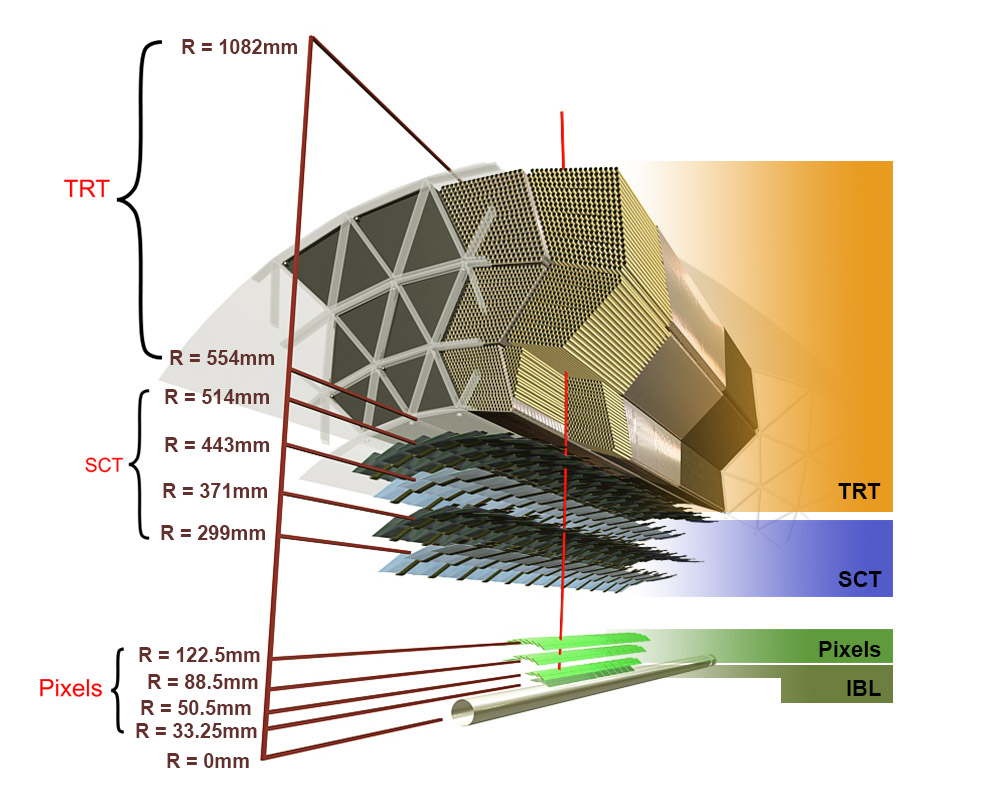
\includegraphics[width=.8\textwidth]{figs/detector/ID}
  \caption{The barrel layers of the Pixel, SCT, and TRT detectors making up the Inner Detector.}
  \label{fig:detector_ID}
\end{figure}

\subsubsection{Pixel Detector} \label{sec:pixel}
The Pixel Detector consists of four cylindrical barrel layers\footnote{For now, the outer three barrel layers will be covered in conjuction with the endcaps; the innermost layer will be described separately.} and three endcap disks on either side.
It is the innermost subdetector of the ID with coverage up to $|\eta| < 2.5$.
The individual sensors measure $50~\mum\times 400~\mum$ and are installed on the silicon wafers that make up the layers.
All in all, there are 1744 wafers with 80 million readout channels.
The sensors themselves are silicon semiconducting diodes that provide a signal when a charged particle passes through.
The Pixel Detector has the finest resolution of all the ID subdetectors, at $10~\mum$ in the $r$-$\phi$ plane and $40~\mum$ in the $z$ direction.

During the upgrade period prior to Run 2, a new innermost layer was added to the Pixel detector barrel: the Insertable B-Layer (IBL)~\cite{2010.ibl-tdr}.
The IBL lies closest to the interaction point, at a radius of 33.25~cm from the beam line, and it is relied upon to provide high-precision measurements close to the interaction point.
Its addition allows better precision in detecting displaced vertices from $b$-jets, for example.
It consists of 280 silicon pixel modules arranged on 14 staves that run parallel to the beam line.
Each stave consists of 12 two-chip planar modules in the middle ($|\eta| < 2.7$) with four 3D sensors~\cite{2015.ibl-3d} on either side ($2.7 < |\eta| < 3.0$).
The IBL's pixel sensors are $50~\mum\times 250~\mum$ in size and have a resolution of $10~\mum$ in $r$-$\phi$ and $75~\mum$ in $z$~\cite{2016.ibl-resolution}.

\subsubsection{Semiconductor Tracker} \label{sec:sct}
The next subdetector of the ID is the SCT, which has four barrel layers and nine endcap disks per side and provides coverage within $|\eta| < 2.5$.
The SCT operates on the same principle as the Pixel Detector, but the sensitive elements are larger silicon ``strips'' placed on the wafers.
This shape change assissts in covering the larger surface area required by the increasing detector radius.
Each detector layer is actually made up of two layers of wafers, placed back-to-back with an angle of 40~mrad between them.
The resolution in the $r$-$\phi$ plane is very fine at $17~\mum$, but, due to the strip shape, the resolution along $z$ is rather poor at $580~\mum$.

\subsubsection{Transition Radiation Tracker} \label{sec:trt}
The outermost component of the ID is the TRT~\cite{2008.trt-tubes, 2008.trt-barrel, 2008.trt-endcap}, which uses a completely different technology from the Pixel and SCT to identify particle hits.
The TRT is unique in that it combines a drift tube tracker with transition radiation detection for electron identification.
The TRT's sensitive elements are drift tubes (referred to as ``straws'') that are 4~mm in diameter and consists of a cylindrical cathode with an anode wire running through the center.
Each straw is filled with a gas mixture including xenon or argon which provide ionizing radiation when high energy particles pass through them.
The resulting electrons drift to the anode and register a voltage, indicating a hit in the detector element.

Between the straws are polyethelene fibers in the barrel and polypropylene foil in the endcaps in order to encourage particles to emit transition radiation photons.
These photons also ionize the gas within the straws, leading to a higher signal.
The TRT takes advantage of the fact that lighter particles are more likely to emit transition radiation by using a ternary output: zero, low-threshold, and high-threshold.
High-threshold hits are generally caused by electrons due to their low mass, and this can help in discriminating electrons against backgrounds. 

There are over 100,000 straws in the barrel of the TRT, and nearly 250,000 in the endcaps.
The TRT provides pseudorapidity coverage up to $|\eta < 2.0|$ with a resolution in the $r$-$\phi$ plane of $130~\mum$.
Since the drift tubes are insensitive along the direction of the wire, the TRT has no resolution in the $z$ direction.
